\documentclass[hide notes,intlimits,usenames,dvipsnames]{beamer}

\mode<presentation>
{
  \usetheme{Singapore}
  \usefonttheme{professionalfonts}
  \setbeamertemplate{blocks}[rounded][shadow=true]
  \setbeamercovered{transparent}
  \setbeamertemplate{footline}[frame number]
}

% load packages
\usepackage[english]{babel}
\usepackage[latin1]{inputenc}
\usepackage[T1]{fontenc}
\usepackage{lmodern}
\usepackage[multidot]{grffile}
\usepackage{verbatim,empheq}

\usepackage{tikz}
\usetikzlibrary{shapes,arrows,shadows}
\usetikzlibrary{decorations.pathreplacing}

\usepackage{animate}
\usepackage{amsmath,verbatim}

\usepackage[noend]{algpseudocode}
\usepackage{listings}

% see http://tex.stackexchange.com/questions/86188/labelling-with-arrows-in-an-automated-way

\newif\ifclipme\clipmetrue
\tikzset{labelstyle/.style={LabelStyle/.append style={#1}},linestyle/.style={LineStyle/.append style={#1}}}
\tikzset{LabelStyle/.initial={},LineStyle/.initial={}}

\newcommand{\mathWithDescription}[4][]{{%
    \tikzset{#1}%
    \tikz[baseline]{
        \node[draw=red,rounded corners,anchor=base] (m#4) {$\displaystyle#2$};
        \ifclipme\begin{pgfinterruptboundingbox}\fi
            \node[above of=m#4,font=\strut, LabelStyle] (l#4) {#3};
            \draw[-,red, LineStyle] (l#4) to (m#4);
        \ifclipme\end{pgfinterruptboundingbox}\fi
    }%
}}

\newcommand{\mathWithDescriptionStarred}[3][]{{%
    \clipmefalse%
    \mathWithDescription[#1]{#2}{#3}{\themathLabelNode}%
}}

\newcounter{mathLabelNode}

\newcommand{\mathLabelBox}[3][]{%
   \stepcounter{mathLabelNode}%
   \mathWithDescription[#1]{#2}{#3}{\themathLabelNode}%
   \vphantom{\mathWithDescriptionStarred[#1]{#2}{#3}{\themathLabelNode}}%
}

\definecolor{dark red}{HTML}{E41A1C}
\definecolor{dark green}{HTML}{4DAF4A}
\definecolor{dark violet}{HTML}{984EA3}
\definecolor{dark blue}{HTML}{084594}
\definecolor{dark orange}{HTML}{FF7F00}
\definecolor{light blue}{HTML}{377EB8}
\definecolor{light red}{HTML}{FB9A99}
\definecolor{light violet}{HTML}{CAB2D6}

\newcommand{\CC}{\mathbb{C}}
\newcommand{\NN}{\mathbb{N}}
\newcommand{\RR}{\mathbb{R}}
\newcommand{\ZZ}{\mathbb{Z}}

\newcommand{\Kcal}{\mathcal{K}}
\newcommand{\Xcal}{\mathcal{X}}

\newcommand{\bF}{\mathbf{F}}
\newcommand{\bQ}{\mathbf{Q}}
\newcommand{\bU}{\mathbf{U}}
\newcommand{\bX}{\mathbf{X}}

\newcommand{\bb}{\mathbf{b}}
\newcommand{\bq}{\mathbf{q}}
\newcommand{\br}{\mathbf{r}}
\newcommand{\bu}{\mathbf{u}}
\newcommand{\bv}{\mathbf{v}}
\newcommand{\bw}{\mathbf{w}}
\newcommand{\bx}{\mathbf{x}}
\newcommand{\by}{\mathbf{y}}
\newcommand{\bz}{\mathbf{z}}

\newcommand{\Div}{\nabla\cdot}
\newcommand{\eps}{\epsilon}
\newcommand{\grad}{\nabla}
\newcommand{\lap}{\triangle}
\renewcommand{\bar}{\overline}

\newcommand{\ip}[2]{\ensuremath{\left<#1,#2\right>}}


\newenvironment{transbox}[1][]{%
\begin{tikzpicture}
\node[drop shadow,rounded corners,text width=\textwidth,fill=white, fill opacity=#1,text opacity=1] \bgroup
}{
\egroup;\end{tikzpicture}}


\title{Optimal solvers for partial differential equations}

\author[Bueler]{Ed Bueler}

\institute[UAF]{
  \scriptsize Dept of Mathematics and Statistics and Geophysical Institute \\

  University of Alaska Fairbanks
}

%\titlegraphic{\includegraphics[width=\textwidth]{andycoast.png}}

\beamertemplatenavigationsymbolsempty   % remove faint and silly navigation symbols at bottom
\renewcommand{\insertnavigation}[1]{}   % remove section headings from top of each slide

\setbeamerfont{date}{size=\scriptsize}
\date{}

\AtBeginSection[]
{
  \begin{frame}<beamer>
    \frametitle{Outline}
    %\tableofcontents[currentsection,hideallsubsections]
    \tableofcontents[currentsection]
  \end{frame}
}


\begin{document}

%\graphicspath{{../../old/commonfigs/}}

\begin{frame}
    \vspace{10mm}
    \titlepage
    \begin{center}
    \tiny DMS Colloquium \quad 28 November, 2017
    \end{center}
\end{frame}

%\begin{frame}
%    \frametitle{Outline}
%    \tableofcontents
%\end{frame}


\section{how to approximately solve a PDE}

%\begin{frame}{ice sheet flows and their boundaries}
%\begin{columns}
%\begin{column}{0.45\textwidth}
%\begin{itemize}
%\item surface slope is discontinuous at grounded margins
%\end{itemize}
%\end{column}
%\begin{column}{0.55\textwidth}
%FIXME
%\end{column}
%\end{columns}
%\end{frame}


\begin{frame}{example: Poisson equation}

\begin{itemize}
\item for most of this talk I'll use just two examples

\bigskip
\item[\textbf{1.}] \emph{Poisson equation} with Dirichlet boundary conditions:
	    $$- \grad^2 u = f \qquad \text{ on } \Omega \subset \RR^d \text{ with } u\big|_{\partial \Omega} = g,$$
    \vspace{-5mm}
	\begin{itemize}
	\item[$\circ$] a linear elliptic PDE problem in dimension $d=2$ or $d=3$
	\item[$\circ$] recall that $\grad^2 u = \Div \left(\grad u\right) = u_{xx}+u_{yy}+u_{zz}$
	\item[$\circ$] source $f(x,y,z)$ given
	\item[$\circ$] boundary values $g(x,y,z)$ given
	\item[$\circ$] will use various domains $\Omega$ including a square, a cube, and
		\begin{itemize}
        \item a snowflake fractal \hspace{0.3in} \begin{tikzpicture}[scale=1.2,baseline] \input{tikz/snowflake.tex} \end{tikzpicture}
        \end{itemize}
	\end{itemize}
\end{itemize}
\end{frame}


\begin{frame}{example: minimal surface equation}

\begin{itemize}
\item[\textbf{2.}] \emph{minimal surface equation (MSE)} with Dirichlet b.c.s:
	    $$- \grad\cdot \left(\frac{\grad u}{\sqrt{1 + |\grad u|^2}}\right) = 0  \qquad \text{ with } u\big|_{\partial \Omega} = g.$$
    \vspace{-2mm}
	\begin{itemize}
	\item[$\circ$] a nonlinear elliptic PDE in 2D
	\item[$\circ$] here on a square domain $\Omega = [0,1]^2$
	\item[$\circ$] the solution $u(x,y)$ gives the height of a zero-gravity soap bubble which spans a wire frame with height $z=g(x,y)$:
	\end{itemize}

\begin{center}
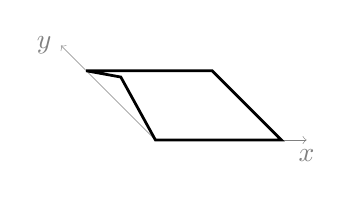
\begin{tikzpicture}[scale=1.6]
  \draw[->,gray,very thin] (0.0,0.0) -- (1.2,0.0) node[below] {$x$};
  \draw[->,gray,very thin] (0.0,0.0) -- (-0.75,0.75) node[left] {$y$};
  \draw[line width=1.0pt] (0.0,0.0) -- (1.0,0.0) -- (0.45,0.55) -- (-0.55,0.55) -- (-0.275,0.5) -- cycle;
\end{tikzpicture}
\end{center}

\vspace{-2mm}
\item both examples 1 \& 2:
	\begin{itemize}
	\item[$\circ$] are well-posed PDE BVPs
	\item[$\circ$] derivable from variational principles
	\item[$\circ$] seek $u \in H_g^1(\Omega)$ \dots from an \alert{$\infty$-dimensional vector space}
	\end{itemize}
\end{itemize}
\end{frame}


\begin{frame}{approximation: finite difference method}
\begin{itemize}
\item a PDE BVP is a system of $\infty$ equations in $\infty$ unknowns
\item some problems can be solved exactly
	\begin{itemize}
	\item[$\circ$] \emph{example}.  $u(x,y)=x^2-y^2$ solves $-\grad^2 u = 0$
	\end{itemize}
\item most problems are not solved exactly, so we
	\begin{itemize}
	\item[$\circ$] \alert{approximate by $N$ equations in $N$ unknowns}
	\item[$\circ$] \dots where $N \ll \infty$
	\end{itemize}
\item one method is \emph{finite differences} (FDM), based on
	    $$f'(x) = \lim_{h \to 0} \frac{f(x+h)-f(x)}{h} \approx \frac{f(x+h)-f(x)}{h}$$
\item in 2D this approximation is used for the Poisson equation:
	    $$u_{xx}+u_{yy} \approx \frac{u_{i+1,j} + u_{i-1,j} + u_{i,j+1} + u_{i,j-1} - 4 u_{ij}}{h^2}$$
	\vspace{-4mm}
	\begin{itemize}
	\item[$\circ$] this assumes the grid has equal spacing $h$ in $x$ and $y$
	\item[$\circ$] similar formula in 3D
	\end{itemize}
\end{itemize}
\end{frame}


\begin{frame}{structured grids}
\begin{itemize}
\item for a majority of this talk I'll use \emph{structured grids}
	\begin{itemize}
	\item[$\circ$] used in all FDM examples
	\end{itemize}
\item in fact, I'll use a sequence of grids $\Omega^{(k)}$
\item the \emph{level} $k$ grid has
	\begin{itemize}
	\item[$\circ$] equal spacing $h_k$ in each direction
	\item[$\circ$] ``increasing resolution'' meaning $h_k \to 0$
    \item[$\circ$] $N_k = O(h_k^{-d}) \to \infty$ points
	    \begin{itemize}
	    \item typically: $N_{k+1} = 2^d N_k$ or nearly so
	    \end{itemize}
    %\item[$\circ$] the coarsest grid is denoted $\Omega^{(0)}$
	\end{itemize}

\bigskip
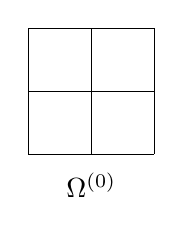
\begin{tikzpicture}[scale=1.6]
  \pgfmathsetmacro\half{1.0/2.0}
  \draw[xstep=\half,ystep=\half,black,thin] (0.0,0.0) grid (1.0,1.0);
  \node at (0.5,-0.25) {$\Omega^{(0)}$};
\end{tikzpicture}
\quad
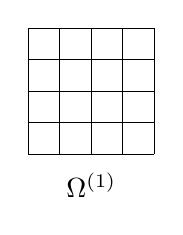
\begin{tikzpicture}[scale=1.6]
  \pgfmathsetmacro\fourth{1.0/4.0}
  \draw[xstep=\fourth,ystep=\fourth,black,thin] (0.0,0.0) grid (1.0,1.0);
  \node at (0.5,-0.25) {$\Omega^{(1)}$};
\end{tikzpicture}
\quad
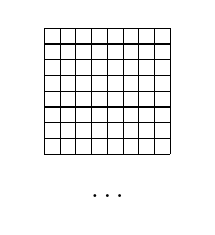
\begin{tikzpicture}[scale=1.6]
  \pgfmathsetmacro\eigth{1.0/8.0}
  \draw[xstep=\eigth,ystep=\eigth,black,thin] (0.0,0.0) grid (1.0,1.0);
  \node at (0.5,-0.25) {$\phantom{\Omega^{(2)}}\dots\phantom{\Omega^{(2)}}$};
\end{tikzpicture}
\quad
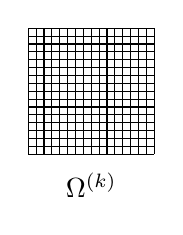
\begin{tikzpicture}[scale=1.6]
  \pgfmathsetmacro\sixteenth{1.0/16.0}
  \draw[xstep=\sixteenth,ystep=\sixteenth,black,thin] (0.0,0.0) grid (1.0,1.0);
  \node at (0.5,-0.25) {$\Omega^{(k)}$};
\end{tikzpicture}

\end{itemize}
\end{frame}


\begin{frame}{approximation: finite element method (FEM)}
\begin{itemize}
\item another way to discretize uses the \emph{weak form} of the PDE
\item for example, the weak form for the Poisson equation comes from integrating-by-parts:
    $$\int_\Omega \grad u \cdot \grad v = \int_\Omega f v \qquad \forall v \in H_0^1(\Omega)$$
\item FEM well-suited to unstructured meshes
\end{itemize}

\begin{center}
\begin{tikzpicture}[scale=1.5,baseline] \input{tikz/snowflake.tex} \end{tikzpicture}
\qquad $\to$ \qquad
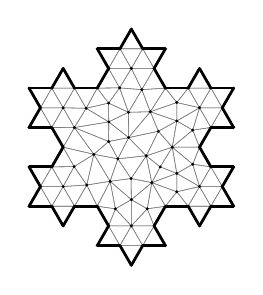
\begin{tikzpicture}[scale=1.5,baseline]   \draw[gray,very thin] (0.346410,0.000000) -- (0.519615,0.144444) -- (0.384900,0.222222) -- (0.346410,0.000000) ;
  \draw[gray,very thin] (-0.024755,0.295315) -- (-0.023014,0.080772) -- (0.160375,0.300000) -- (-0.024755,0.295315) ;
  \draw[gray,very thin] (-0.577350,-0.333333) -- (-0.673575,-0.500000) -- (-0.481125,-0.500000) -- (-0.577350,-0.333333) ;
  \draw[gray,very thin] (-0.866025,-0.500000) -- (-0.673575,-0.500000) -- (-0.769800,-0.333333) -- (-0.866025,-0.500000) ;
  \draw[gray,very thin] (-0.866025,-0.166667) -- (-0.769800,-0.333333) -- (-0.673575,-0.166667) -- (-0.866025,-0.166667) ;
  \draw[gray,very thin] (0.173205,-0.300000) -- (0.000000,-0.444444) -- (0.134715,-0.522222) -- (0.173205,-0.300000) ;
  \draw[gray,very thin] (-0.769800,-0.333333) -- (-0.673575,-0.500000) -- (-0.577350,-0.333333) -- (-0.769800,-0.333333) ;
  \draw[gray,very thin] (0.577350,0.000000) -- (0.673575,0.166667) -- (0.519615,0.144444) -- (0.577350,0.000000) ;
  \draw[gray,very thin] (-0.673575,-0.500000) -- (-0.577350,-0.666667) -- (-0.481125,-0.500000) -- (-0.673575,-0.500000) ;
  \draw[gray,very thin] (0.160375,0.300000) -- (0.384900,0.377778) -- (0.288675,0.500000) -- (0.160375,0.300000) ;
  \draw[gray,very thin] (-0.179620,-0.288889) -- (-0.134715,-0.522222) -- (0.000000,-0.444444) -- (-0.179620,-0.288889) ;
  \draw[gray,very thin] (0.577350,0.333333) -- (0.519615,0.144444) -- (0.673575,0.166667) -- (0.577350,0.333333) ;
  \draw[gray,very thin] (-0.192450,-0.666667) -- (-0.096225,-0.833333) -- (0.000000,-0.666667) -- (-0.192450,-0.666667) ;
  \draw[gray,very thin] (-0.288675,-0.833333) -- (-0.096225,-0.833333) -- (-0.192450,-0.666667) -- (-0.288675,-0.833333) ;
  \draw[gray,very thin] (0.192450,0.666667) -- (0.000000,0.666667) -- (0.088770,0.487087) -- (0.192450,0.666667) ;
  \draw[gray,very thin] (-0.484564,-0.164681) -- (-0.577350,0.000000) -- (-0.673575,-0.166667) -- (-0.484564,-0.164681) ;
  \draw[gray,very thin] (-0.288675,-0.500000) -- (-0.192450,-0.666667) -- (-0.134715,-0.522222) -- (-0.288675,-0.500000) ;
  \draw[gray,very thin] (-0.769800,-0.333333) -- (-0.577350,-0.333333) -- (-0.673575,-0.166667) -- (-0.769800,-0.333333) ;
  \draw[gray,very thin] (0.000000,-0.666667) -- (-0.096225,-0.833333) -- (0.096225,-0.833333) -- (0.000000,-0.666667) ;
  \draw[gray,very thin] (0.000000,-0.666667) -- (-0.134715,-0.522222) -- (-0.192450,-0.666667) -- (0.000000,-0.666667) ;
  \draw[gray,very thin] (0.384900,0.222222) -- (0.228882,0.134801) -- (0.346410,0.000000) -- (0.384900,0.222222) ;
  \draw[gray,very thin] (-0.377445,-0.320420) -- (-0.577350,-0.333333) -- (-0.481125,-0.500000) -- (-0.377445,-0.320420) ;
  \draw[gray,very thin] (0.173205,-0.300000) -- (0.134715,-0.522222) -- (0.288675,-0.500000) -- (0.173205,-0.300000) ;
  \draw[gray,very thin] (-0.002300,-0.265618) -- (0.173205,-0.300000) -- (0.126543,-0.073060) -- (-0.002300,-0.265618) ;
  \draw[gray,very thin] (-0.769800,0.333333) -- (-0.673575,0.166667) -- (-0.577350,0.333333) -- (-0.769800,0.333333) ;
  \draw[gray,very thin] (-0.866025,0.166667) -- (-0.673575,0.166667) -- (-0.769800,0.333333) -- (-0.866025,0.166667) ;
  \draw[gray,very thin] (-0.866025,0.500000) -- (-0.769800,0.333333) -- (-0.673575,0.500000) -- (-0.866025,0.500000) ;
  \draw[gray,very thin] (0.288675,-0.500000) -- (0.384900,-0.377778) -- (0.173205,-0.300000) -- (0.288675,-0.500000) ;
  \draw[gray,very thin] (-0.673575,0.500000) -- (-0.769800,0.333333) -- (-0.577350,0.333333) -- (-0.673575,0.500000) ;
  \draw[gray,very thin] (0.000000,-0.666667) -- (0.134715,-0.522222) -- (0.000000,-0.444444) -- (0.000000,-0.666667) ;
  \draw[gray,very thin] (-0.481125,0.500000) -- (-0.673575,0.500000) -- (-0.577350,0.333333) -- (-0.481125,0.500000) ;
  \draw[gray,very thin] (-0.482235,0.166026) -- (-0.317460,-0.060428) -- (-0.192007,0.048135) -- (-0.482235,0.166026) ;
  \draw[gray,very thin] (0.384900,-0.377778) -- (0.577350,-0.333333) -- (0.384900,-0.222222) -- (0.384900,-0.377778) ;
  \draw[gray,very thin] (-0.481125,0.500000) -- (-0.577350,0.666667) -- (-0.673575,0.500000) -- (-0.481125,0.500000) ;
  \draw[gray,very thin] (-0.577350,0.333333) -- (-0.382627,0.329396) -- (-0.481125,0.500000) -- (-0.577350,0.333333) ;
  \draw[gray,very thin] (-0.577350,0.000000) -- (-0.482235,0.166026) -- (-0.673575,0.166667) -- (-0.577350,0.000000) ;
  \draw[gray,very thin] (-0.288675,0.833333) -- (-0.192450,0.666667) -- (-0.096225,0.833333) -- (-0.288675,0.833333) ;
  \draw[gray,very thin] (-0.377445,-0.320420) -- (-0.481125,-0.500000) -- (-0.288675,-0.500000) -- (-0.377445,-0.320420) ;
  \draw[gray,very thin] (-0.096225,0.833333) -- (-0.192450,0.666667) -- (0.000000,0.666667) -- (-0.096225,0.833333) ;
  \draw[gray,very thin] (0.519615,-0.144444) -- (0.577350,-0.333333) -- (0.673575,-0.166667) -- (0.519615,-0.144444) ;
  \draw[gray,very thin] (-0.179620,-0.288889) -- (-0.288675,-0.500000) -- (-0.134715,-0.522222) -- (-0.179620,-0.288889) ;
  \draw[gray,very thin] (0.346410,0.000000) -- (0.384900,-0.222222) -- (0.519615,-0.144444) -- (0.346410,0.000000) ;
  \draw[gray,very thin] (-0.099664,0.501985) -- (-0.192826,0.373078) -- (-0.024755,0.295315) -- (-0.099664,0.501985) ;
  \draw[gray,very thin] (0.384900,0.222222) -- (0.160375,0.300000) -- (0.228882,0.134801) -- (0.384900,0.222222) ;
  \draw[gray,very thin] (-0.096225,-0.833333) -- (0.000000,-1.000000) -- (0.096225,-0.833333) -- (-0.096225,-0.833333) ;
  \draw[gray,very thin] (0.577350,0.333333) -- (0.384900,0.377778) -- (0.384900,0.222222) -- (0.577350,0.333333) ;
  \draw[gray,very thin] (0.096225,-0.833333) -- (0.288675,-0.833333) -- (0.192450,-0.666667) -- (0.096225,-0.833333) ;
  \draw[gray,very thin] (-0.134715,-0.522222) -- (0.000000,-0.666667) -- (0.000000,-0.444444) -- (-0.134715,-0.522222) ;
  \draw[gray,very thin] (0.288675,-0.500000) -- (0.481125,-0.500000) -- (0.384900,-0.377778) -- (0.288675,-0.500000) ;
  \draw[gray,very thin] (0.192450,-0.666667) -- (0.288675,-0.500000) -- (0.134715,-0.522222) -- (0.192450,-0.666667) ;
  \draw[gray,very thin] (-0.099664,0.501985) -- (-0.192450,0.666667) -- (-0.288675,0.500000) -- (-0.099664,0.501985) ;
  \draw[gray,very thin] (0.134715,-0.522222) -- (0.000000,-0.666667) -- (0.192450,-0.666667) -- (0.134715,-0.522222) ;
  \draw[gray,very thin] (0.481125,-0.500000) -- (0.577350,-0.666667) -- (0.673575,-0.500000) -- (0.481125,-0.500000) ;
  \draw[gray,very thin] (0.481125,-0.500000) -- (0.673575,-0.500000) -- (0.577350,-0.333333) -- (0.481125,-0.500000) ;
  \draw[gray,very thin] (0.346410,0.000000) -- (0.126543,-0.073060) -- (0.244503,-0.167073) -- (0.346410,0.000000) ;
  \draw[gray,very thin] (-0.114417,-0.098508) -- (0.126543,-0.073060) -- (-0.023014,0.080772) -- (-0.114417,-0.098508) ;
  \draw[gray,very thin] (0.673575,-0.500000) -- (0.866025,-0.500000) -- (0.769800,-0.333333) -- (0.673575,-0.500000) ;
  \draw[gray,very thin] (0.384900,0.377778) -- (0.160375,0.300000) -- (0.384900,0.222222) -- (0.384900,0.377778) ;
  \draw[gray,very thin] (0.577350,-0.333333) -- (0.519615,-0.144444) -- (0.384900,-0.222222) -- (0.577350,-0.333333) ;
  \draw[gray,very thin] (0.673575,-0.166667) -- (0.577350,-0.333333) -- (0.769800,-0.333333) -- (0.673575,-0.166667) ;
  \draw[gray,very thin] (0.519615,0.144444) -- (0.577350,0.333333) -- (0.384900,0.222222) -- (0.519615,0.144444) ;
  \draw[gray,very thin] (0.519615,-0.144444) -- (0.673575,-0.166667) -- (0.577350,0.000000) -- (0.519615,-0.144444) ;
  \draw[gray,very thin] (0.866025,-0.166667) -- (0.673575,-0.166667) -- (0.769800,-0.333333) -- (0.866025,-0.166667) ;
  \draw[gray,very thin] (0.577350,0.000000) -- (0.519615,0.144444) -- (0.346410,0.000000) -- (0.577350,0.000000) ;
  \draw[gray,very thin] (-0.317460,-0.060428) -- (-0.484564,-0.164681) -- (-0.377445,-0.320420) -- (-0.317460,-0.060428) ;
  \draw[gray,very thin] (0.673575,-0.500000) -- (0.769800,-0.333333) -- (0.577350,-0.333333) -- (0.673575,-0.500000) ;
  \draw[gray,very thin] (0.173205,-0.300000) -- (0.384900,-0.222222) -- (0.244503,-0.167073) -- (0.173205,-0.300000) ;
  \draw[gray,very thin] (-0.317460,-0.060428) -- (-0.577350,0.000000) -- (-0.484564,-0.164681) -- (-0.317460,-0.060428) ;
  \draw[gray,very thin] (-0.577350,-0.333333) -- (-0.377445,-0.320420) -- (-0.484564,-0.164681) -- (-0.577350,-0.333333) ;
  \draw[gray,very thin] (0.000000,0.666667) -- (0.192450,0.666667) -- (0.096225,0.833333) -- (0.000000,0.666667) ;
  \draw[gray,very thin] (0.384900,0.377778) -- (0.481125,0.500000) -- (0.288675,0.500000) -- (0.384900,0.377778) ;
  \draw[gray,very thin] (-0.191155,0.214038) -- (-0.382627,0.329396) -- (-0.482235,0.166026) -- (-0.191155,0.214038) ;
  \draw[gray,very thin] (0.346410,0.000000) -- (0.519615,-0.144444) -- (0.577350,0.000000) -- (0.346410,0.000000) ;
  \draw[gray,very thin] (-0.096225,0.833333) -- (0.096225,0.833333) -- (0.000000,1.000000) -- (-0.096225,0.833333) ;
  \draw[gray,very thin] (0.288675,0.833333) -- (0.096225,0.833333) -- (0.192450,0.666667) -- (0.288675,0.833333) ;
  \draw[gray,very thin] (0.000000,-0.444444) -- (0.173205,-0.300000) -- (-0.002300,-0.265618) -- (0.000000,-0.444444) ;
  \draw[gray,very thin] (0.288675,0.500000) -- (0.088770,0.487087) -- (0.160375,0.300000) -- (0.288675,0.500000) ;
  \draw[gray,very thin] (0.000000,0.666667) -- (0.096225,0.833333) -- (-0.096225,0.833333) -- (0.000000,0.666667) ;
  \draw[gray,very thin] (0.673575,0.166667) -- (0.866025,0.166667) -- (0.769800,0.333333) -- (0.673575,0.166667) ;
  \draw[gray,very thin] (0.384900,0.377778) -- (0.577350,0.333333) -- (0.481125,0.500000) -- (0.384900,0.377778) ;
  \draw[gray,very thin] (0.173205,-0.300000) -- (0.384900,-0.377778) -- (0.384900,-0.222222) -- (0.173205,-0.300000) ;
  \draw[gray,very thin] (0.673575,0.500000) -- (0.481125,0.500000) -- (0.577350,0.333333) -- (0.673575,0.500000) ;
  \draw[gray,very thin] (0.577350,-0.333333) -- (0.384900,-0.377778) -- (0.481125,-0.500000) -- (0.577350,-0.333333) ;
  \draw[gray,very thin] (0.577350,0.666667) -- (0.481125,0.500000) -- (0.673575,0.500000) -- (0.577350,0.666667) ;
  \draw[gray,very thin] (0.866025,0.500000) -- (0.673575,0.500000) -- (0.769800,0.333333) -- (0.866025,0.500000) ;
  \draw[gray,very thin] (-0.002300,-0.265618) -- (-0.179620,-0.288889) -- (0.000000,-0.444444) -- (-0.002300,-0.265618) ;
  \draw[gray,very thin] (-0.192826,0.373078) -- (-0.099664,0.501985) -- (-0.288675,0.500000) -- (-0.192826,0.373078) ;
  \draw[gray,very thin] (0.769800,0.333333) -- (0.673575,0.500000) -- (0.577350,0.333333) -- (0.769800,0.333333) ;
  \draw[gray,very thin] (0.769800,0.333333) -- (0.577350,0.333333) -- (0.673575,0.166667) -- (0.769800,0.333333) ;
  \draw[gray,very thin] (-0.377445,-0.320420) -- (-0.179620,-0.288889) -- (-0.317460,-0.060428) -- (-0.377445,-0.320420) ;
  \draw[gray,very thin] (-0.577350,-0.333333) -- (-0.484564,-0.164681) -- (-0.673575,-0.166667) -- (-0.577350,-0.333333) ;
  \draw[gray,very thin] (0.192450,-0.666667) -- (0.000000,-0.666667) -- (0.096225,-0.833333) -- (0.192450,-0.666667) ;
  \draw[gray,very thin] (0.126543,-0.073060) -- (-0.114417,-0.098508) -- (-0.002300,-0.265618) -- (0.126543,-0.073060) ;
  \draw[gray,very thin] (-0.288675,-0.500000) -- (-0.179620,-0.288889) -- (-0.377445,-0.320420) -- (-0.288675,-0.500000) ;
  \draw[gray,very thin] (0.192450,0.666667) -- (0.088770,0.487087) -- (0.288675,0.500000) -- (0.192450,0.666667) ;
  \draw[gray,very thin] (0.000000,0.666667) -- (-0.192450,0.666667) -- (-0.099664,0.501985) -- (0.000000,0.666667) ;
  \draw[gray,very thin] (-0.192826,0.373078) -- (-0.288675,0.500000) -- (-0.382627,0.329396) -- (-0.192826,0.373078) ;
  \draw[gray,very thin] (0.000000,0.666667) -- (-0.099664,0.501985) -- (0.088770,0.487087) -- (0.000000,0.666667) ;
  \draw[gray,very thin] (-0.002300,-0.265618) -- (-0.114417,-0.098508) -- (-0.179620,-0.288889) -- (-0.002300,-0.265618) ;
  \draw[gray,very thin] (0.088770,0.487087) -- (-0.099664,0.501985) -- (-0.024755,0.295315) -- (0.088770,0.487087) ;
  \draw[gray,very thin] (-0.288675,0.500000) -- (-0.481125,0.500000) -- (-0.382627,0.329396) -- (-0.288675,0.500000) ;
  \draw[gray,very thin] (-0.024755,0.295315) -- (-0.192826,0.373078) -- (-0.191155,0.214038) -- (-0.024755,0.295315) ;
  \draw[gray,very thin] (-0.577350,0.333333) -- (-0.673575,0.166667) -- (-0.482235,0.166026) -- (-0.577350,0.333333) ;
  \draw[gray,very thin] (-0.191155,0.214038) -- (-0.192826,0.373078) -- (-0.382627,0.329396) -- (-0.191155,0.214038) ;
  \draw[gray,very thin] (-0.023014,0.080772) -- (-0.024755,0.295315) -- (-0.191155,0.214038) -- (-0.023014,0.080772) ;
  \draw[gray,very thin] (0.088770,0.487087) -- (-0.024755,0.295315) -- (0.160375,0.300000) -- (0.088770,0.487087) ;
  \draw[gray,very thin] (-0.317460,-0.060428) -- (-0.482235,0.166026) -- (-0.577350,0.000000) -- (-0.317460,-0.060428) ;
  \draw[gray,very thin] (-0.577350,0.333333) -- (-0.482235,0.166026) -- (-0.382627,0.329396) -- (-0.577350,0.333333) ;
  \draw[gray,very thin] (-0.191155,0.214038) -- (-0.482235,0.166026) -- (-0.192007,0.048135) -- (-0.191155,0.214038) ;
  \draw[gray,very thin] (-0.023014,0.080772) -- (0.126543,-0.073060) -- (0.228882,0.134801) -- (-0.023014,0.080772) ;
  \draw[gray,very thin] (-0.192007,0.048135) -- (-0.023014,0.080772) -- (-0.191155,0.214038) -- (-0.192007,0.048135) ;
  \draw[gray,very thin] (-0.317460,-0.060428) -- (-0.179620,-0.288889) -- (-0.114417,-0.098508) -- (-0.317460,-0.060428) ;
  \draw[gray,very thin] (-0.317460,-0.060428) -- (-0.114417,-0.098508) -- (-0.192007,0.048135) -- (-0.317460,-0.060428) ;
  \draw[gray,very thin] (-0.023014,0.080772) -- (-0.192007,0.048135) -- (-0.114417,-0.098508) -- (-0.023014,0.080772) ;
  \draw[gray,very thin] (-0.023014,0.080772) -- (0.228882,0.134801) -- (0.160375,0.300000) -- (-0.023014,0.080772) ;
  \draw[gray,very thin] (0.126543,-0.073060) -- (0.346410,0.000000) -- (0.228882,0.134801) -- (0.126543,-0.073060) ;
  \draw[gray,very thin] (0.346410,0.000000) -- (0.244503,-0.167073) -- (0.384900,-0.222222) -- (0.346410,0.000000) ;
  \draw[gray,very thin] (0.126543,-0.073060) -- (0.173205,-0.300000) -- (0.244503,-0.167073) -- (0.126543,-0.073060) ;
  \filldraw (-0.866025,0.500000) circle (0.200000pt);
  \filldraw (-0.673575,0.500000) circle (0.200000pt);
  \filldraw (-0.577350,0.666667) circle (0.200000pt);
  \filldraw (-0.481125,0.500000) circle (0.200000pt);
  \filldraw (-0.288675,0.500000) circle (0.200000pt);
  \filldraw (-0.192450,0.666667) circle (0.200000pt);
  \filldraw (-0.288675,0.833333) circle (0.200000pt);
  \filldraw (-0.096225,0.833333) circle (0.200000pt);
  \filldraw (0.000000,1.000000) circle (0.200000pt);
  \filldraw (0.096225,0.833333) circle (0.200000pt);
  \filldraw (0.288675,0.833333) circle (0.200000pt);
  \filldraw (0.192450,0.666667) circle (0.200000pt);
  \filldraw (0.288675,0.500000) circle (0.200000pt);
  \filldraw (0.481125,0.500000) circle (0.200000pt);
  \filldraw (0.577350,0.666667) circle (0.200000pt);
  \filldraw (0.673575,0.500000) circle (0.200000pt);
  \filldraw (0.866025,0.500000) circle (0.200000pt);
  \filldraw (0.769800,0.333333) circle (0.200000pt);
  \filldraw (0.866025,0.166667) circle (0.200000pt);
  \filldraw (0.673575,0.166667) circle (0.200000pt);
  \filldraw (0.577350,0.000000) circle (0.200000pt);
  \filldraw (0.673575,-0.166667) circle (0.200000pt);
  \filldraw (0.866025,-0.166667) circle (0.200000pt);
  \filldraw (0.769800,-0.333333) circle (0.200000pt);
  \filldraw (0.866025,-0.500000) circle (0.200000pt);
  \filldraw (0.673575,-0.500000) circle (0.200000pt);
  \filldraw (0.577350,-0.666667) circle (0.200000pt);
  \filldraw (0.481125,-0.500000) circle (0.200000pt);
  \filldraw (0.288675,-0.500000) circle (0.200000pt);
  \filldraw (0.192450,-0.666667) circle (0.200000pt);
  \filldraw (0.288675,-0.833333) circle (0.200000pt);
  \filldraw (0.096225,-0.833333) circle (0.200000pt);
  \filldraw (0.000000,-1.000000) circle (0.200000pt);
  \filldraw (-0.096225,-0.833333) circle (0.200000pt);
  \filldraw (-0.288675,-0.833333) circle (0.200000pt);
  \filldraw (-0.192450,-0.666667) circle (0.200000pt);
  \filldraw (-0.288675,-0.500000) circle (0.200000pt);
  \filldraw (-0.481125,-0.500000) circle (0.200000pt);
  \filldraw (-0.577350,-0.666667) circle (0.200000pt);
  \filldraw (-0.673575,-0.500000) circle (0.200000pt);
  \filldraw (-0.866025,-0.500000) circle (0.200000pt);
  \filldraw (-0.769800,-0.333333) circle (0.200000pt);
  \filldraw (-0.866025,-0.166667) circle (0.200000pt);
  \filldraw (-0.673575,-0.166667) circle (0.200000pt);
  \filldraw (-0.577350,0.000000) circle (0.200000pt);
  \filldraw (-0.673575,0.166667) circle (0.200000pt);
  \filldraw (-0.866025,0.166667) circle (0.200000pt);
  \filldraw (-0.769800,0.333333) circle (0.200000pt);
  \filldraw (-0.577350,-0.333333) circle (0.200000pt);
  \filldraw (0.000000,-0.444444) circle (0.200000pt);
  \filldraw (-0.577350,0.333333) circle (0.200000pt);
  \filldraw (0.000000,0.666667) circle (0.200000pt);
  \filldraw (0.384900,-0.222222) circle (0.200000pt);
  \filldraw (0.577350,-0.333333) circle (0.200000pt);
  \filldraw (0.384900,0.222222) circle (0.200000pt);
  \filldraw (0.577350,0.333333) circle (0.200000pt);
  \filldraw (0.000000,-0.666667) circle (0.200000pt);
  \filldraw (-0.134715,-0.522222) circle (0.200000pt);
  \filldraw (-0.179620,-0.288889) circle (0.200000pt);
  \filldraw (0.134715,-0.522222) circle (0.200000pt);
  \filldraw (0.173205,-0.300000) circle (0.200000pt);
  \filldraw (0.384900,-0.377778) circle (0.200000pt);
  \filldraw (0.519615,-0.144444) circle (0.200000pt);
  \filldraw (0.346410,0.000000) circle (0.200000pt);
  \filldraw (0.519615,0.144444) circle (0.200000pt);
  \filldraw (0.384900,0.377778) circle (0.200000pt);
  \filldraw (0.160375,0.300000) circle (0.200000pt);
  \filldraw (-0.377445,-0.320420) circle (0.200000pt);
  \filldraw (-0.317460,-0.060428) circle (0.200000pt);
  \filldraw (-0.484564,-0.164681) circle (0.200000pt);
  \filldraw (-0.002300,-0.265618) circle (0.200000pt);
  \filldraw (0.126543,-0.073060) circle (0.200000pt);
  \filldraw (0.088770,0.487087) circle (0.200000pt);
  \filldraw (-0.099664,0.501985) circle (0.200000pt);
  \filldraw (-0.191155,0.214038) circle (0.200000pt);
  \filldraw (-0.192826,0.373078) circle (0.200000pt);
  \filldraw (-0.382627,0.329396) circle (0.200000pt);
  \filldraw (-0.024755,0.295315) circle (0.200000pt);
  \filldraw (-0.482235,0.166026) circle (0.200000pt);
  \filldraw (-0.023014,0.080772) circle (0.200000pt);
  \filldraw (-0.114417,-0.098508) circle (0.200000pt);
  \filldraw (-0.192007,0.048135) circle (0.200000pt);
  \filldraw (0.228882,0.134801) circle (0.200000pt);
  \filldraw (0.244503,-0.167073) circle (0.200000pt);
  \draw[line width=1.000000pt] (-0.673575,0.500000) -- (-0.866025,0.500000);
  \draw[line width=1.000000pt] (-0.673575,0.500000) -- (-0.577350,0.666667);
  \draw[line width=1.000000pt] (-0.481125,0.500000) -- (-0.577350,0.666667);
  \draw[line width=1.000000pt] (-0.288675,0.500000) -- (-0.481125,0.500000);
  \draw[line width=1.000000pt] (-0.288675,0.500000) -- (-0.192450,0.666667);
  \draw[line width=1.000000pt] (-0.192450,0.666667) -- (-0.288675,0.833333);
  \draw[line width=1.000000pt] (-0.288675,0.833333) -- (-0.096225,0.833333);
  \draw[line width=1.000000pt] (-0.096225,0.833333) -- (0.000000,1.000000);
  \draw[line width=1.000000pt] (0.096225,0.833333) -- (0.000000,1.000000);
  \draw[line width=1.000000pt] (0.096225,0.833333) -- (0.288675,0.833333);
  \draw[line width=1.000000pt] (0.192450,0.666667) -- (0.288675,0.833333);
  \draw[line width=1.000000pt] (0.192450,0.666667) -- (0.288675,0.500000);
  \draw[line width=1.000000pt] (0.481125,0.500000) -- (0.288675,0.500000);
  \draw[line width=1.000000pt] (0.481125,0.500000) -- (0.577350,0.666667);
  \draw[line width=1.000000pt] (0.577350,0.666667) -- (0.673575,0.500000);
  \draw[line width=1.000000pt] (0.673575,0.500000) -- (0.866025,0.500000);
  \draw[line width=1.000000pt] (0.866025,0.500000) -- (0.769800,0.333333);
  \draw[line width=1.000000pt] (0.769800,0.333333) -- (0.866025,0.166667);
  \draw[line width=1.000000pt] (0.866025,0.166667) -- (0.673575,0.166667);
  \draw[line width=1.000000pt] (0.673575,0.166667) -- (0.577350,0.000000);
  \draw[line width=1.000000pt] (0.673575,-0.166667) -- (0.577350,0.000000);
  \draw[line width=1.000000pt] (0.673575,-0.166667) -- (0.866025,-0.166667);
  \draw[line width=1.000000pt] (0.866025,-0.166667) -- (0.769800,-0.333333);
  \draw[line width=1.000000pt] (0.769800,-0.333333) -- (0.866025,-0.500000);
  \draw[line width=1.000000pt] (0.866025,-0.500000) -- (0.673575,-0.500000);
  \draw[line width=1.000000pt] (0.673575,-0.500000) -- (0.577350,-0.666667);
  \draw[line width=1.000000pt] (0.577350,-0.666667) -- (0.481125,-0.500000);
  \draw[line width=1.000000pt] (0.481125,-0.500000) -- (0.288675,-0.500000);
  \draw[line width=1.000000pt] (0.288675,-0.500000) -- (0.192450,-0.666667);
  \draw[line width=1.000000pt] (0.192450,-0.666667) -- (0.288675,-0.833333);
  \draw[line width=1.000000pt] (0.288675,-0.833333) -- (0.096225,-0.833333);
  \draw[line width=1.000000pt] (0.096225,-0.833333) -- (0.000000,-1.000000);
  \draw[line width=1.000000pt] (0.000000,-1.000000) -- (-0.096225,-0.833333);
  \draw[line width=1.000000pt] (-0.288675,-0.833333) -- (-0.096225,-0.833333);
  \draw[line width=1.000000pt] (-0.192450,-0.666667) -- (-0.288675,-0.833333);
  \draw[line width=1.000000pt] (-0.192450,-0.666667) -- (-0.288675,-0.500000);
  \draw[line width=1.000000pt] (-0.481125,-0.500000) -- (-0.288675,-0.500000);
  \draw[line width=1.000000pt] (-0.481125,-0.500000) -- (-0.577350,-0.666667);
  \draw[line width=1.000000pt] (-0.577350,-0.666667) -- (-0.673575,-0.500000);
  \draw[line width=1.000000pt] (-0.866025,-0.500000) -- (-0.673575,-0.500000);
  \draw[line width=1.000000pt] (-0.769800,-0.333333) -- (-0.866025,-0.500000);
  \draw[line width=1.000000pt] (-0.769800,-0.333333) -- (-0.866025,-0.166667);
  \draw[line width=1.000000pt] (-0.673575,-0.166667) -- (-0.866025,-0.166667);
  \draw[line width=1.000000pt] (-0.673575,-0.166667) -- (-0.577350,0.000000);
  \draw[line width=1.000000pt] (-0.577350,0.000000) -- (-0.673575,0.166667);
  \draw[line width=1.000000pt] (-0.673575,0.166667) -- (-0.866025,0.166667);
  \draw[line width=1.000000pt] (-0.769800,0.333333) -- (-0.866025,0.166667);
  \draw[line width=1.000000pt] (-0.769800,0.333333) -- (-0.866025,0.500000);
 \end{tikzpicture}
\end{center}
\end{frame}


\begin{frame}{approximation: finite element method}
\begin{itemize}
\item \dots and an $N$-dimensional subspace $\mathcal{X}_N \subset H^1(\Omega)$,
\item \dots and a basis of \emph{tent functions} $\psi_i(x,y)$ FIXME show tent
\item by supposing [2D] $u(x,y) = \sum_j u_{j} \psi_{j}(x,y)$ and requiring $\ast$ for all $v=\psi_i$ we get system of $N$ eqns in $N$ unknowns
\end{itemize}
\end{frame}


\begin{frame}{linear systems with sparse matrices}
\begin{itemize}
\item FDM and FEM produce FIXME
\end{itemize}

\includegraphics[width=\textwidth]{figs/spythree}
\end{frame}


\begin{frame}{FIXME}
\begin{itemize}
\item FIXME  SPD?
\end{itemize}
\end{frame}


\section{what is an ``optimal solver''?}

\begin{frame}{define ``optimal''}
\begin{itemize}
\item consider $N$ equations in $N$ unknowns $\mathbf{F}(\mathbf{u}) = 0$
	\begin{itemize}
	\item[$\circ$] $\mathbf{F}:\RR^N \to \RR^N$, the \emph{residual}, is generally nonlinear
	\item[$\circ$] but $\mathbf{F}(\mathbf{w}) = \mathbf{b} - A \mathbf{w}$ is the linear case
	\end{itemize}
\item for FDM and FEM discretizations of a PDE, evaluating $\mathbf{F}(\mathbf{w})$, for given $\mathbf{w}$, requires $O(N)$ work

\bigskip
\indent \item[\textbf{def.}]  an algorithm which solves $\mathbf{F}(\mathbf{u}) = 0$ is \emph{optimal} if it does $O(N)$ or $O(N\log N)$ work

\bigskip
\item  ``solves'' means that it generates $\mathbf{u}_n$ so that
	    $$\frac{\|\mathbf{F}(\mathbf{u}_n)\|}{\|\mathbf{F}(\mathbf{u}_0)\|} \le \text{tol}$$
where $\mathbf{u}_0$ is an initial guess
\end{itemize}
\end{frame}

\begin{frame}{example: solving tridiagonal matrices}
\begin{itemize}
\item FIXME
\end{itemize}
\end{frame}

\begin{frame}{non-example:  banded Gaussian elimination (2D,3D)}
\begin{itemize}
\item FIXME
\end{itemize}
\end{frame}

\begin{frame}{tangent: spectral methods}
\begin{itemize}
\item FIXME
\item spectral methods show that pursuit of optimality is \emph{not} the only good goal
\end{itemize}
\end{frame}

\begin{frame}{Krylov methods}
\begin{itemize}
\item FIXME
\end{itemize}
\end{frame}

\begin{frame}{rate of convergence of CG}
\begin{itemize}
\item FIXME
\end{itemize}
\end{frame}


\section{multigrid}

\begin{frame}{multigrid: what it does}

\small
\begin{itemize}
\item given structured grids $\left\{\Omega^{(j)}\right\}_0^k$
\item given initial guess $\bu_0$ on the finest grid $\Omega^{(k)}$
\item basic multigrid cycle to solve $A \bu = \bb$ is $\text{\textsc{Vcycle}}(\bu_0,k)$:

\medskip
\begin{algorithmic}
\footnotesize
\Function{Vcycle}{$\bw,l$}
    \If{$l == 0$}
        \State solve $A \bv = \bb$, e.g.~by a direct solver
    \Else
        \State improve $\bw$ on the level $l$ grid, giving $\bv$
        \State compute residual $\br = \bb - A \bv$
        \State restrict $\br$ to level $l-1$, giving $\br^C$
        \State $\bz^C = \text{\textsc{Vcycle}}(0,l-1$)
        \State $\bv \gets \bv + (\text{interpolate } \bz^C \text{ to level $l$ grid})$
        \State improve $\bv$ some more on the level $l$ grid
        \EndIf
    \Return $\bv$
\EndFunction
\end{algorithmic}
\end{itemize}
\end{frame}


\begin{frame}{multigrid V-cycles}

\begin{itemize}
\item FIXME
\end{itemize}

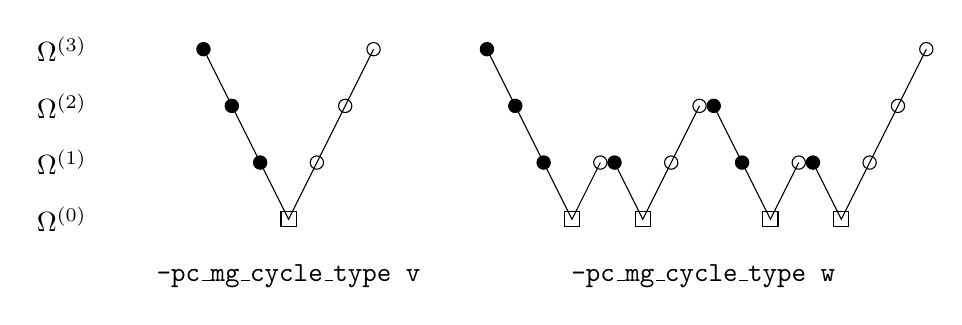
\begin{tikzpicture}[scale=1.2]
% see also fullcycle.tex

  \pgfmathsetmacro\hstep{0.3}
  \pgfmathsetmacro\vstep{0.6}
  \pgfmathsetmacro\ceps{0.08}   % size of square for coarse grid

% grid labels at left
  \node at (-1.5,3*\vstep) {$\Omega^{(3)}$};
  \node at (-1.5,2*\vstep) {$\Omega^{(2)}$};
  \node at (-1.5,\vstep) {$\Omega^{(1)}$};
  \node at (-1.5,0.0) {$\Omega^{(0)}$};

% V-cycle
  \draw[black,thin] (0.0,3*\vstep) -- (\hstep,2*\vstep) --  (2*\hstep,\vstep) -- (3*\hstep,0.0)
                    -- (4*\hstep,\vstep) -- (5*\hstep,2*\vstep) -- (6*\hstep,3*\vstep);
  \filldraw (0.0,3*\vstep) circle (2.0pt);
  \filldraw (\hstep,2*\vstep) circle (2.0pt);
  \filldraw (2*\hstep,\vstep) circle (2.0pt);
  \draw     (3*\hstep-\ceps,-\ceps) rectangle (3*\hstep+\ceps,+\ceps);
  \draw     (4*\hstep,\vstep) circle (2.0pt);
  \draw     (5*\hstep,2*\vstep) circle (2.0pt);
  \draw     (6*\hstep,3*\vstep) circle (2.0pt);

% W-cycle
  \pgfmathsetmacro\woff{10*\hstep}
  \draw[shift={(\woff,0)},black,thin] (0.0,3*\vstep) -- (\hstep,2*\vstep) --  (2*\hstep,\vstep) -- (3*\hstep,0.0)
                    -- (4*\hstep,\vstep);
  \draw[shift={(\woff,0)},black,thin] (4.5*\hstep,\vstep) -- (5.5*\hstep,0.0) -- (6.5*\hstep,\vstep) --  (7.5*\hstep,2*\vstep);
  \draw[shift={(\woff,0)},black,thin] (8*\hstep,2*\vstep) -- (9*\hstep,\vstep) --  (10*\hstep,0.0) -- (11*\hstep,\vstep);
  \draw[shift={(\woff,0)},black,thin] (11.5*\hstep,\vstep) -- (12.5*\hstep,0.0) -- (13.5*\hstep,\vstep) -- (14.5*\hstep,2*\vstep) -- (15.5*\hstep,3*\vstep);
  \filldraw[shift={(\woff,0)}] (0.0,3*\vstep) circle (2.0pt);
  \filldraw[shift={(\woff,0)}] (\hstep,2*\vstep) circle (2.0pt);
  \filldraw[shift={(\woff,0)}] (2*\hstep,\vstep) circle (2.0pt);
  \draw[shift={(\woff,0)}]     (3*\hstep-\ceps,-\ceps) rectangle (3*\hstep+\ceps,+\ceps);
  \draw[shift={(\woff,0)}]     (4*\hstep,\vstep) circle (2.0pt);
  \filldraw[shift={(\woff,0)}] (4.5*\hstep,\vstep) circle (2.0pt);
  \draw[shift={(\woff,0)}]     (5.5*\hstep-\ceps,-\ceps) rectangle (5.5*\hstep+\ceps,+\ceps);
  \draw[shift={(\woff,0)}]     (6.5*\hstep,\vstep) circle (2.0pt);
  \draw[shift={(\woff,0)}]     (7.5*\hstep,2*\vstep) circle (2.0pt);
  \filldraw[shift={(\woff,0)}] (8.0*\hstep,2*\vstep) circle (2.0pt);
  \filldraw[shift={(\woff,0)}] (9.0*\hstep,\vstep) circle (2.0pt);
  \draw[shift={(\woff,0)}]     (10.0*\hstep-\ceps,-\ceps) rectangle (10.0*\hstep+\ceps,+\ceps);
  \draw[shift={(\woff,0)}]     (11.0*\hstep,\vstep) circle (2.0pt);
  \filldraw[shift={(\woff,0)}] (11.5*\hstep,\vstep) circle (2.0pt);
  \draw[shift={(\woff,0)}]     (12.5*\hstep-\ceps,-\ceps) rectangle (12.5*\hstep+\ceps,+\ceps);
  \draw[shift={(\woff,0)}]     (13.5*\hstep,\vstep) circle (2.0pt);
  \draw[shift={(\woff,0)}]     (14.5*\hstep,2*\vstep) circle (2.0pt);
  \draw[shift={(\woff,0)}]     (15.5*\hstep,3*\vstep) circle (2.0pt);

% option labels
  \node at (3*\hstep,-0.6) {\texttt{-pc\_mg\_cycle\_type v}};
  \node[shift={(\woff,0)}] at (9.3*\hstep,-0.6) {\texttt{-pc\_mg\_cycle\_type w}};

\end{tikzpicture}




\medskip
\qquad 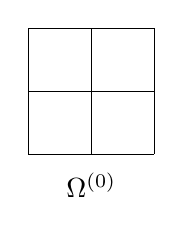
\begin{tikzpicture}[scale=1.6]
  \pgfmathsetmacro\half{1.0/2.0}
  \draw[xstep=\half,ystep=\half,black,thin] (0.0,0.0) grid (1.0,1.0);
  \node at (0.5,-0.25) {$\Omega^{(0)}$};
\end{tikzpicture}
\quad
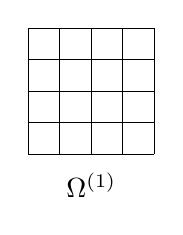
\begin{tikzpicture}[scale=1.6]
  \pgfmathsetmacro\fourth{1.0/4.0}
  \draw[xstep=\fourth,ystep=\fourth,black,thin] (0.0,0.0) grid (1.0,1.0);
  \node at (0.5,-0.25) {$\Omega^{(1)}$};
\end{tikzpicture}
\quad
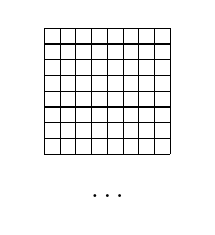
\begin{tikzpicture}[scale=1.6]
  \pgfmathsetmacro\eigth{1.0/8.0}
  \draw[xstep=\eigth,ystep=\eigth,black,thin] (0.0,0.0) grid (1.0,1.0);
  \node at (0.5,-0.25) {$\phantom{\Omega^{(2)}}\dots\phantom{\Omega^{(2)}}$};
\end{tikzpicture}
\quad
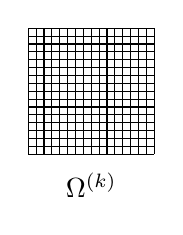
\begin{tikzpicture}[scale=1.6]
  \pgfmathsetmacro\sixteenth{1.0/16.0}
  \draw[xstep=\sixteenth,ystep=\sixteenth,black,thin] (0.0,0.0) grid (1.0,1.0);
  \node at (0.5,-0.25) {$\Omega^{(k)}$};
\end{tikzpicture}

\end{frame}


\begin{frame}{multigrid: why it works}
\begin{itemize}
\item FIXME
\end{itemize}
\end{frame}


\begin{frame}{an optimality lemma}

conditions under which multgrid cycles as preconditioners for CG give optimal solver
\begin{itemize}
\item FIXME
\end{itemize}
\end{frame}


\section{nonlinear problems and unstructured grids}

\begin{frame}{FIXME}
\begin{itemize}
\item FIXME
\end{itemize}
\end{frame}



\section{barriers to optimality}


\begin{frame}{low regularity of solution}
\begin{itemize}
\item again assume solution of (nonlinear) BVP on $\Omega \subset \RR^d$
\item $W(h)$ Newton iterations
\item $K(h)$ preconditioned Krylov steps per Newton
\item FIXME  in some case number of Newton steps (or Krylov steps) now grows as $h\to 0$
\item can demo w MSE
\end{itemize}
\end{frame}


\begin{frame}{constrained problem}
\begin{itemize}
\item FIXME  number of Newton steps proportional to $D/h$ where $D$ is distance-to-move free boundary
\item Max working on it
\end{itemize}
\end{frame}


\begin{frame}{initial/boundary value problems}

\begin{itemize}
\item problem posed on $\Omega \times [0,T]$ where $\Omega \subset \RR^d$
    \begin{itemize}
    \item[$\circ$] example: nonlinear convection/diffusion/reaction equation
      $$u_t = \Div(a(u) \grad u) - b(u)\cdot \grad u + f(u)$$
    \item[$\circ$] evolution problem with states in some $W_k^p(\Omega)$
    \end{itemize}
\item for these problems there's no intrinsic ``barrier'' \dots
\item rather a lack of clarity about what ``optimal'' should mean
\end{itemize}
\end{frame}


\begin{frame}{numerical parameters for IBVPs}

\begin{itemize}
\item assume structured grid: $h=\Delta x = \Delta y=\Delta z$
    \begin{itemize}
    \item[$\circ$] $N=$ (spatial degrees of freedom) $=O(h^{-d})$
    \end{itemize}
\item time step is limited in some way \dots almost always:
    $$\Delta t \le O(h^q)$$
    \vspace{-5mm}
    \begin{itemize}
    \item[$\circ$] stability: $q=2$ for explicit schemes on diffusions
	    \begin{itemize}
	    \item explicit schemes clearly not optimal
	    \end{itemize}
    \item[$\circ$] accuracy: usually $q=1$
	    \begin{itemize}
	    \item e.g.~for $O(h^2+\Delta t^2)$ methods
	    \end{itemize}
    \item[$\circ$] movie: generate $M$ frames, so $\Delta t = T/M$
    \item[$\circ$] ``total number of degrees of freedom'' $=M N$?
    \end{itemize}
\item (implicit) solution for one time step using NK:
    \begin{itemize}
    \item[$\circ$] $W(h)$ Newton iterations
    \item[$\circ$] $K(h)$ preconditioned Krylov steps per Newton
    \item[$\circ$] $W(h)=K(h)=1$ for explicit methods
    \end{itemize}
\end{itemize}
\end{frame}


\begin{frame}{optimality(?) for IBVPs}

\begin{itemize}
\item yields: a ``performance model'' for solving IBVPs on $\Omega \times [0,T]$
\item cost of computation:
\footnotesize
\begin{align*}
C &= (\text{number of steps}) \cdot (\text{iterations per step}) \cdot (\text{cost of 1 spatial residual}) \\
  &= O(h^{-q}) \cdot W(h) \, K(h) \cdot O(h^{-d})
\end{align*}
\normalsize
\item we define solver to be \emph{optimal} if work is $O(MN)$?
    \begin{itemize}
    \item[$\circ$] optimal movie-limited (implicit) steps:
        $$C = M \cdot W \cdot O(1) \cdot O(h^{-d}) = O(MN)$$
    \item[$\circ$] optimal accuracy-limited (implicit) steps:
        $$C = O(h^{-1}) \cdot W \cdot O(1) \cdot O(h^{-d}) = O(N^{1+1/d})$$
    \item[$\circ$] explicit:
        $$C = O(h^{-2}) \cdot 1 \cdot 1 \cdot O(h^{-d}) = O(N^{1+2/d}) \hfill \alert{\leftarrow \text{ beat this!?}}$$
    \end{itemize}
\end{itemize}
\end{frame}


\begin{frame}{goal of parallel scaling}
\begin{itemize}
\item FIXME not exactly a ``barrier'' but a conflict
\end{itemize}
\end{frame}


\begin{frame}{conclusion}
\begin{itemize}
\item as you head toward $N=\infty$, in approximately solving your PDE-type problem on a modern computer,

\bigskip
\begin{quote}
\alert{you should be able to solve $N$ equations in $N$ unknowns in $O(N)$ time!}
\end{quote}

\bigskip
\item it is a good goal, anyway
\end{itemize}
\end{frame}


\end{document}
